\part{Calculos Manuales}

La presnete seccion tiene como objetivo modelar una ataguia utilizando redes de flujo y lineas equipotenciales graficadas $"$a mano $"$ a travez de python. De esta manera, se buscaran calcular factores como el caudal de infiltracion,
la presion de poros a lo largo de la ataguia, la estabilidad, falla por licuefaccion y factor de seguridad. Todos estas calculos fueron realizados mediante python, de esta manera, se pudo efectuar un analisis mas exausto y preciso en los distintos casos.

\section{Teoria}
\subsection{Líneas de Flujo}
Las líneas de flujo representan las trayectorias que siguen las partículas de agua al moverse a través de un medio poroso. En un diagrama de flujo, estas líneas son perpendiculares a las líneas equipotenciales y muestran la dirección del flujo subterráneo o de infiltración. En estructuras como las ataguías, las líneas de flujo se usan para predecir el comportamiento del agua alrededor y debajo de la estructura, ayudando a diseñar sistemas eficaces de control de agua. \textbf{\cite{structville}}

\subsection{Líneas Equipotenciales}
Las líneas equipotenciales representan ubicaciones con igual carga hidráulica, lo que significa que no hay diferencia de energía a lo largo de ellas. En problemas de flujo de agua subterránea, como los relacionados con las ataguías, estas líneas ayudan a visualizar la distribución de la energía potencial dentro del agua. Son fundamentales para determinar el caudal de agua y asegurar que esta no desestabilice estructuras como los diques o presas. \textbf{\cite{structville}}

\subsection{Caudal de infiltracion}

El caudal de infiltración es el flujo de agua que penetra a través del suelo, debido a la diferencia de presión entre el nivel de agua dentro y fuera de la ataguía en este caso. La tasa de infiltración esta condicionada por la permeabilidad del suelo y la diferencia de carga hidráulica. Para poder calcular el caudal de infiltración, se utiliza la fórmula (\ref{eq:caudal_infiltracion}). \textbf{\cite{stability_cofferdam_2024}}

\begin{equation}
    Q = k \cdot \frac{\Delta H}{N_{f}} \cdot N_{d}
    \label{eq:caudal_infiltracion}
\end{equation}

Donde:
\begin{itemize}
    \item $Q$ = Caudal de Infiltracion
    \item $k$ = Coeficiente de permeabilidad
    \item $\Delta H$ = Diferencia de carga hidraulica
    \item $N_{f}$ = Cantidad de canales de flujo
    \item $N_{d}$ = Cantidad de canales equipotenciales
\end{itemize}

\subsection{Presión de Poros}
La presión de poros es la fuerza que el agua ejerce dentro de los poros de un material como el suelo o la roca. Juega un papel crucial en la construcción con agua o alto nivel freático, ya que una presión de poros excesiva puede reducir el esfuerzo efectivo en el suelo, lo que podría ocasionar problemas como la licuefacción, donde el suelo pierde firmeza, o la formación de tuberías subterráneas. En las ataguías, la presión de poros es un factor clave, ya que afecta la estabilidad del terreno que rodea la estructura. Para poder calcular la presión de poros, se utiliza la siguiente formula. \textbf{\cite{jeas}}

\begin{equation}
    u = \gamma \cdot h
    \label{eq:presion_poros}
\end{equation}

Donde:
\begin{itemize}
    \item $u$ = Presión de Poros
    \item $\gamma$ = Peso Específico del Agua
    \item $h$ = Profundidad del agua
\end{itemize}


\subsection{Gradiente Hidráulico}
El gradiente hidráulico es el cambio de la carga hidráulica por unidad de distancia en la dirección del flujo. Es un factor crucial para determinar el flujo de agua a través de suelos. En el diseño de ataguías, el gradiente hidráulico ayuda a predecir problemas como la licuefacción, donde los gradientes elevados pueden erosionar el suelo y causar fallos estructurales. Este se calcula con la formula (\ref{eq:gradiente_hidraulico}). \textbf{\cite{budhu_soil_2010}}
\begin{equation}
    i = \frac{\Delta h}{\Delta L}
    \label{eq:gradiente_hidraulico}
\end{equation}
Donde:
\begin{itemize}
    \item $i$ = Gradiente Hidráulico
    \item $\Delta h$ = Cambio de carga hidráulica
    \item $\Delta L$ = Distancia en la dirección del flujo
\end{itemize}
\subsubsection{Licuefacción}
La licuefacción se genera cuando se excede el gradiente hidráulico crítico (\ref{eq:gradiente_critico}), lo que provoca que el suelo pierda su capacidad de soporte y se comporte como un líquido. En el diseño de ataguías, la licuefacción es un problema grave, ya que puede causar el colapso de la estructura y daños significativos a la infraestructura circundante. \textbf{\cite{budhu_soil_2010}}

\begin{equation}
    i_{critico} = \frac{\Delta h}{L_{min}}
    \label{eq:gradiente_critico}
\end{equation}

\subsection{Presión en una Ataguía}
La presión dentro y alrededor de una ataguía es resultado tanto del nivel de agua como de las condiciones del suelo. El diseño de una ataguía implica calcular la caída de carga potencial, la presión de poros y el gradiente hidráulico, lo que permite predecir si la estructura soportará las presiones del agua y del suelo que actúan sobre ella. Las redes de flujo se utilizan para evaluar estas presiones y estimar la infiltración de agua a través de la cimentación. \cite{sivakugan2005}

\section{Resultados}

\subsection{Diagramas Escala 1:200}

\begin{figure}[H]
    \centering
    \begin{minipage}{0.32\textwidth}
        \centering
        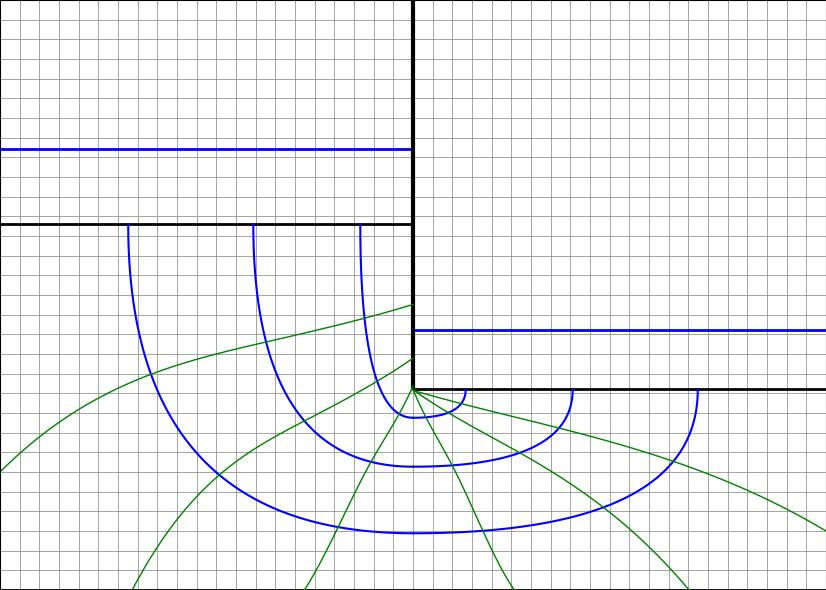
\includegraphics[width=\textwidth]{GRAFICOS/caso_1.jpg}
        \caption{Caso 1}
        \label{fig:caso_1}
    \end{minipage}
    \begin{minipage}{0.32\textwidth}
        \centering
        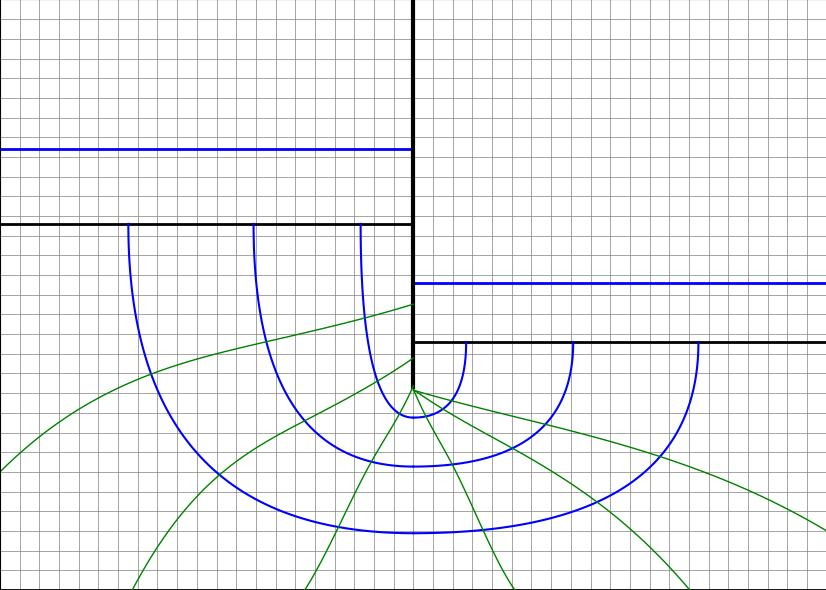
\includegraphics[width=\textwidth]{GRAFICOS/caso_2.jpg}
        \caption{Caso 2}
        \label{fig:caso_2}
    \end{minipage}
    \begin{minipage}{0.32\textwidth}
        \centering
        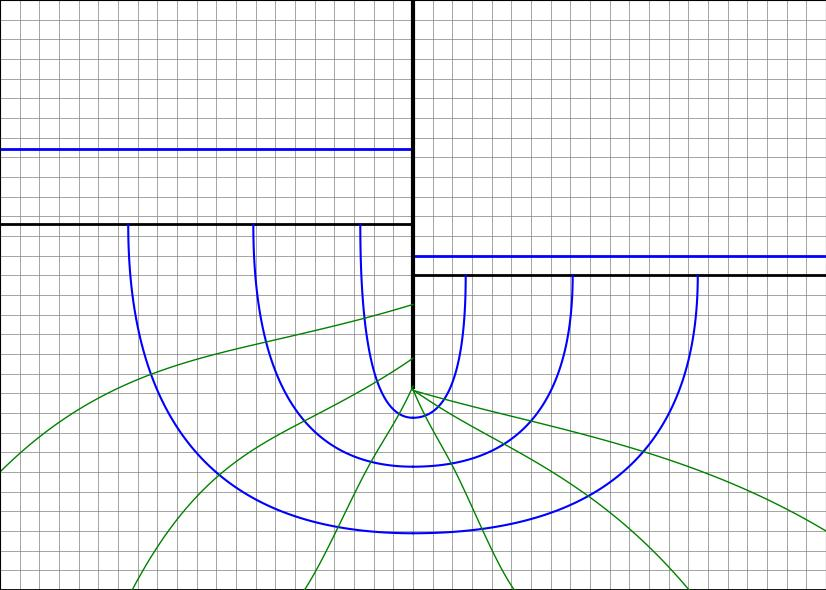
\includegraphics[width=\textwidth]{GRAFICOS/caso_3.jpg}
        \caption{Caso 3}
        \label{fig:caso_3}
    \end{minipage}
  \end{figure}

Para poder visualizar los 3 casos de ataguías, se graficaron los diagramas a escala 1:200. En estos se pueden observar las líneas de flujo (azules) y equipotenciales (verdes), las cuales permiten visualizar el comportamiento del agua alrededor de la ataguía. Es importante señalar, que para el caso 1 el agua tiene que recorrer una menor distancia para llegar al otro lado de la ataguía, lo que se traduce en una mayor cantidad de agua infiltrada. Por otro lado, el caso 3 es el que presenta una mayor longitud de linea de flujo, lo que se traduce en una menor cantidad de agua infiltrada.

\subsection{Presion de Poros}
Para poder calcular la presión de poros para cada caso se utilizó la formula (\ref{eq:presion_poros}). 
\subsubsection{Distribucion Presiones}

\begin{figure}[H]
    \centering
    \begin{minipage}{0.32\textwidth}
        \centering
        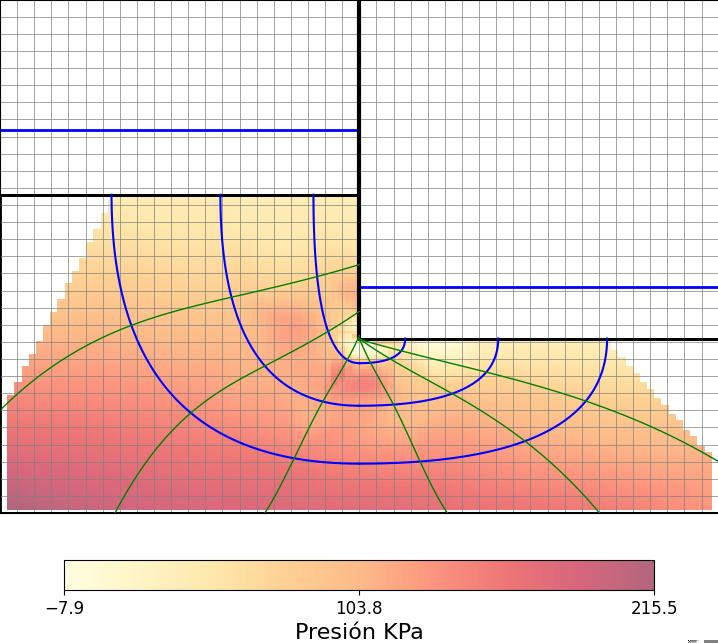
\includegraphics[width=\textwidth]{GRAFICOS/caso_1_presion_poros.jpg}
        \caption{Caso 1 Presion Poros}
        \label{fig:caso_1_presion_poros}
    \end{minipage}
    \begin{minipage}{0.32\textwidth}
        \centering
        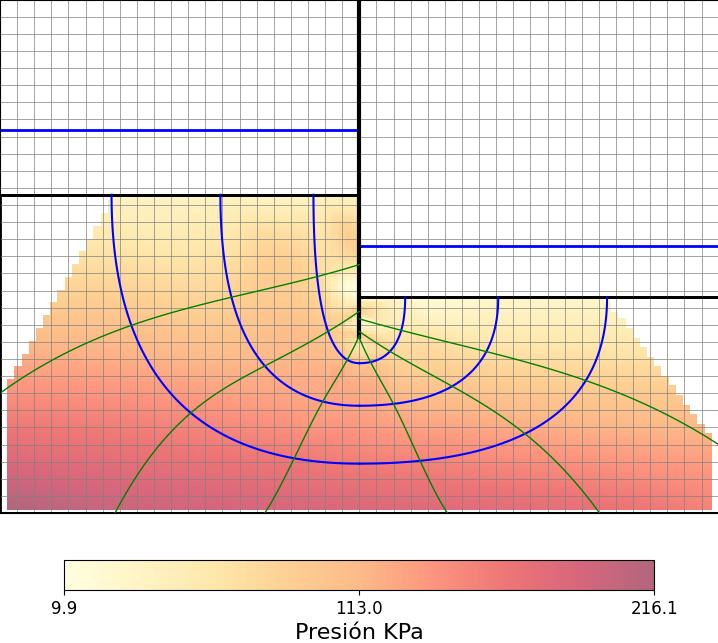
\includegraphics[width=\textwidth]{GRAFICOS/caso_2_presion_poros.jpg}
        \caption{Caso 2 Presion Poros}
        \label{fig:caso_2_presion_poros}
    \end{minipage}
    \begin{minipage}{0.32\textwidth}
        \centering
        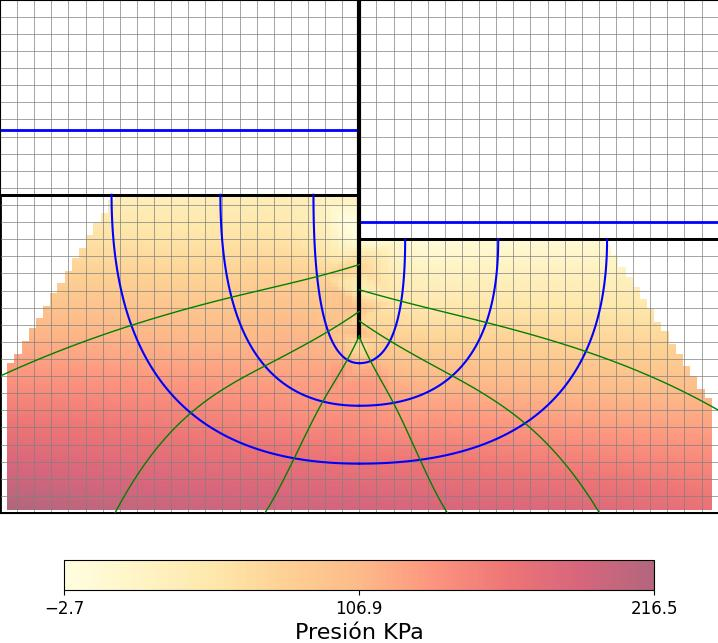
\includegraphics[width=\textwidth]{GRAFICOS/caso_3_presion_poros.jpg}
        \caption{Caso 3 Presion Poros}
        \label{fig:caso_3_presion_poros}
    \end{minipage}
\end{figure}

Como se puede observar, para el caso \ref{fig:caso_1_presion_poros} en la parte inferior de la ataguía se presenta una mayor presión de poros que en los otros dos casos, lo que se traduce en una mayor cantidad de agua infiltrada y un mayor rieso de licuefacción. Por otro lado, en los casos \ref{fig:caso_2_presion_poros} y \ref{fig:caso_3_presion_poros} se observa que la presión de poros es menor en la parte inferior de la ataguía, lo que se traduce en una menor cantidad de agua infiltrada haciendo más estable y segura la estructura.

\subsubsection{Presiones Totales}

\begin{figure}[H]
    \centering
    \begin{minipage}{0.32\textwidth}
        \centering
        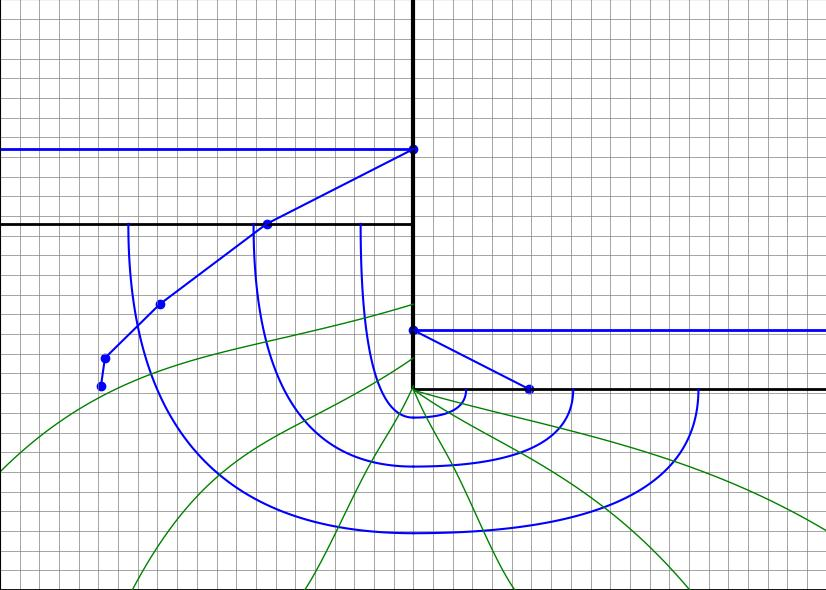
\includegraphics[width=\textwidth]{GRAFICOS/caso_1_presion_ataguia_total.jpg}
        \caption{Caso 1 Presion Ataguia Total}
        \label{fig:caso_1_presion_ataguia_total}
    \end{minipage}
    \begin{minipage}{0.32\textwidth}
        \centering
        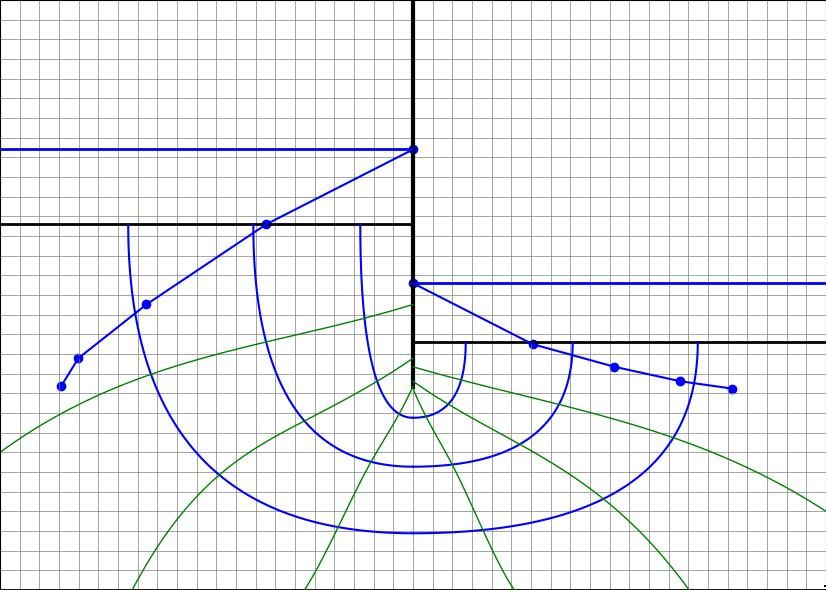
\includegraphics[width=\textwidth]{GRAFICOS/caso_2_presion_ataguia_total.jpg}
        \caption{Caso 2 Presion Ataguia Total}
        \label{fig:caso_2_presion_ataguia_total}
    \end{minipage}
    \begin{minipage}{0.32\textwidth}
        \centering
        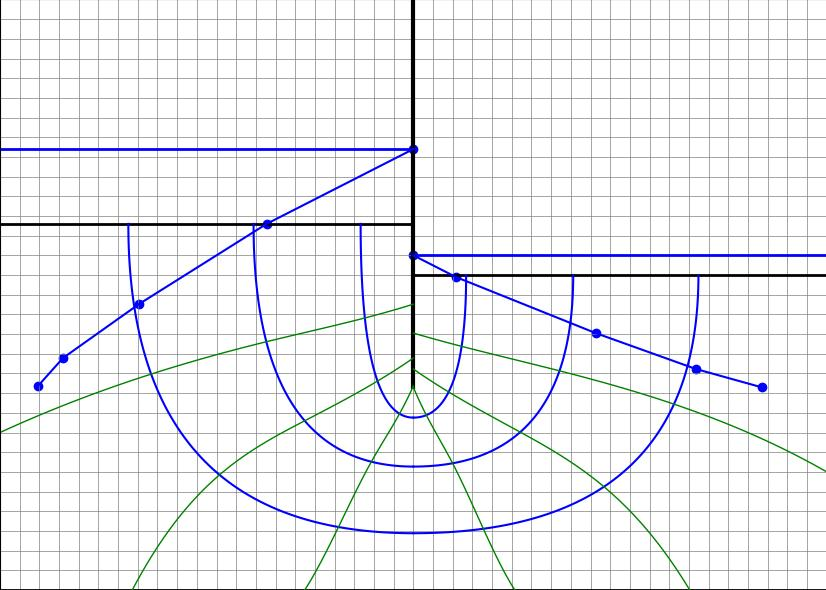
\includegraphics[width=\textwidth]{GRAFICOS/caso_3_presion_ataguia_total.jpg}
        \caption{Caso 3 Presion Ataguia Total}
        \label{fig:caso_3_presion_ataguia_total}
    \end{minipage}
\end{figure}

En los diagramas de presión total, se puede observar que para todos los casos la presión en la parte derecha de la ataguía es igual, sin embargo, en la parte derecha a medida que el nivel del suelo aumenta, esta también aumenta. Esto se puede ver en el caso \ref{fig:caso_1_presion_ataguia_total} que la presión en el lado derecho es bajo, mientras que en el caso \ref{fig:caso_3_presion_ataguia_total} la presión es mayor. Los efectos de esto se pueden observar en las presiones efectivas.

\subsubsection{Presiones Efectivas}

Para poder apreciar de mejor manera el efecto de las presiones en la ataguía se diagramaron las presiones efectivas, esto se calcula restando la presión del lado derecho con la presión del lado izquierdo. 

\begin{figure}[H]
    \centering
    \begin{minipage}{0.32\textwidth}
        \centering
        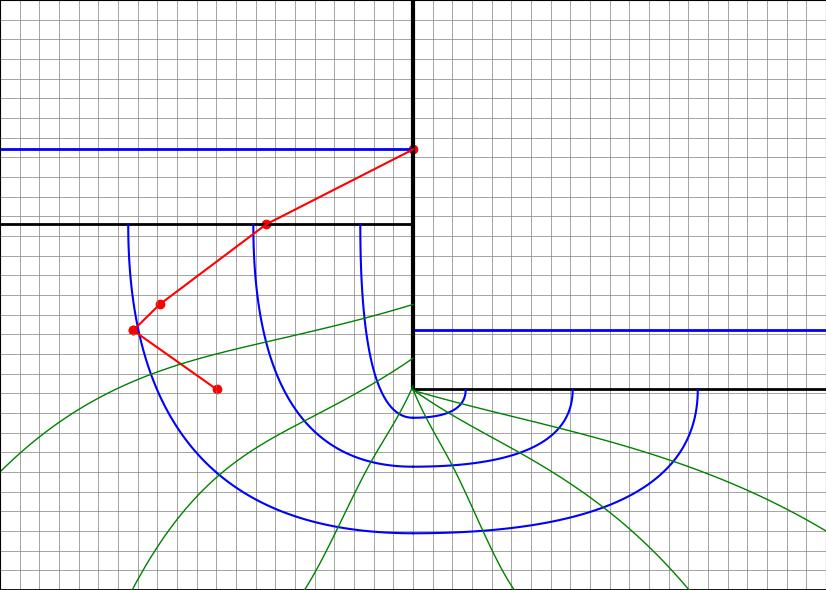
\includegraphics[width=\textwidth]{GRAFICOS/caso_1_presion_ataguia_neta.jpg}
        \caption{Caso 1 Presion Ataguia Neta}
        \label{fig:caso_1_presion_ataguia_neta}
    \end{minipage}
    \begin{minipage}{0.32\textwidth}
        \centering
        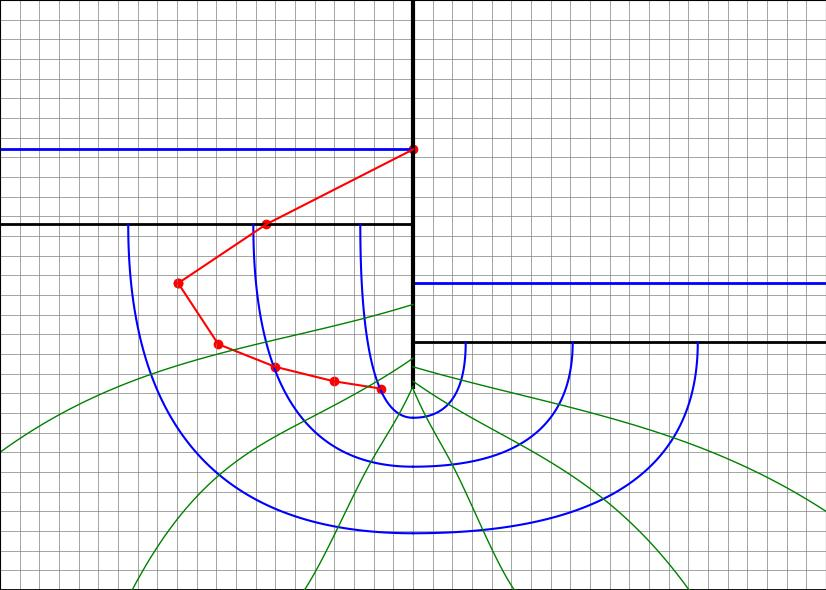
\includegraphics[width=\textwidth]{GRAFICOS/caso_2_presion_ataguia_neta.jpg}
        \caption{Caso 2 Presion Ataguia Neta}
        \label{fig:caso_2_presion_ataguia_neta}
    \end{minipage}
    \begin{minipage}{0.32\textwidth}
        \centering
        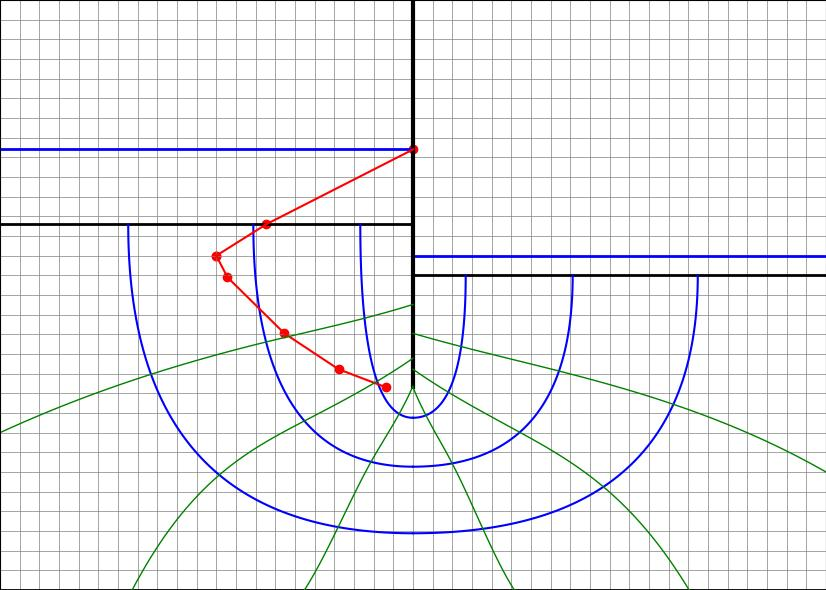
\includegraphics[width=\textwidth]{GRAFICOS/caso_3_presion_ataguia_neta.jpg}
        \caption{Caso 3 Presion Ataguia Neta}
        \label{fig:caso_3_presion_ataguia_neta}
    \end{minipage}
\end{figure}

Como se puede observar, a medida que el nivel del suelo va subiendo, la presión en el fondo de la ataguía va disminuyendo, lo que se traduce en una menor presión efectiva. Esto se puede observar en el caso \ref{fig:caso_1_presion_ataguia_neta} donde la presión efectiva es mayor en la parte inferior de la ataguía, mientras que en el caso \ref{fig:caso_3_presion_ataguia_neta} la presión efectiva es menor.

\subsubsection{Estabilidad}
Finalmente, para poder determinar la estabilidad de la ataguía se calculó el centroide de la ataguía en cada caso. Esto se hizo en base a las presiones efectivas calculadas anteriormente.
\begin{figure}[H]
    \centering
    \begin{minipage}{0.32\textwidth}
        \centering
        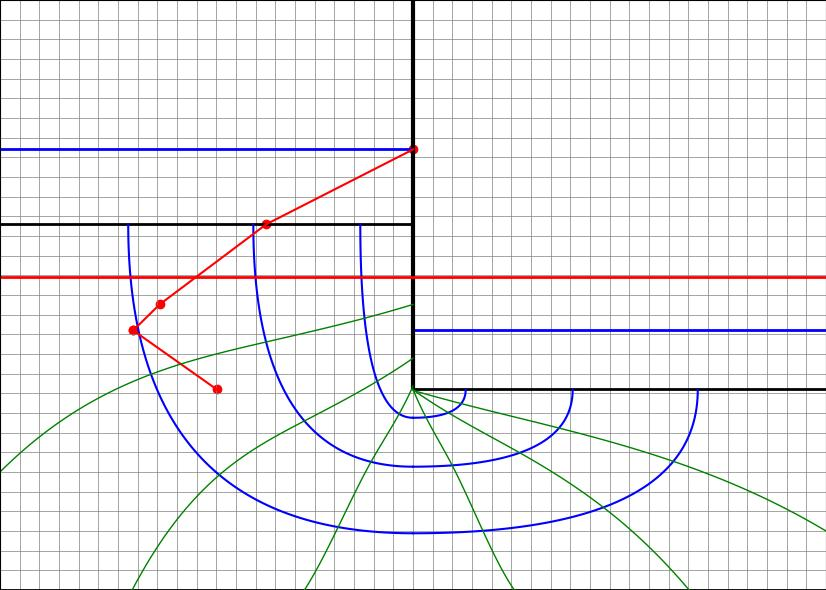
\includegraphics[width=\textwidth]{GRAFICOS/caso_1_centroide_y.jpg}
        \caption{Caso 1 Centroide}
        \label{fig:caso_1_centroide_y}
    \end{minipage}
    \begin{minipage}{0.32\textwidth}
        \centering
        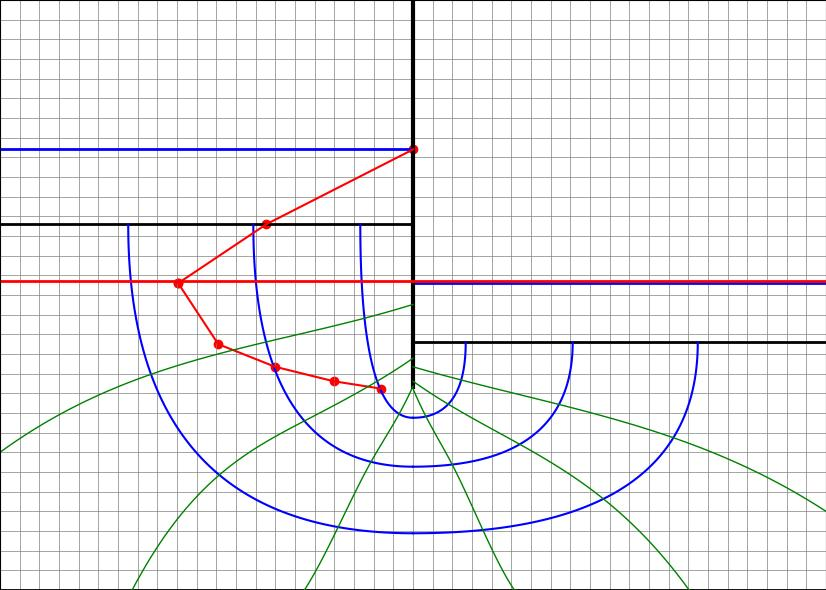
\includegraphics[width=\textwidth]{GRAFICOS/caso_2_centroide_y.jpg}
        \caption{Caso 2 Centroide}
        \label{fig:caso_2_centroide_y}
    \end{minipage}
    \begin{minipage}{0.32\textwidth}
        \centering
        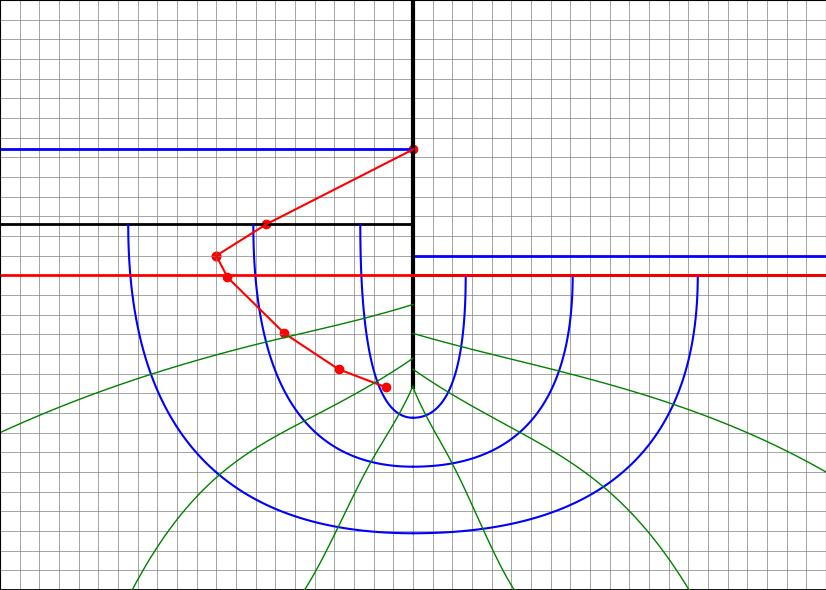
\includegraphics[width=\textwidth]{GRAFICOS/caso_3_centroide_y.jpg}
        \caption{Caso 3 Centroide}
        \label{fig:caso_3_centroide_y}
    \end{minipage}
\end{figure}

Como se puede observar, en el caso \ref{fig:caso_1_centroide_y} el centroide se encuentra en una parte elevada de la ataguía. Esto genera un momento que tiende a voltear la ataguía, lo que conlleva a una menor estabilidad. Luego, a medida que el nivel de agua y suelo van aumentando el centroide se va desplazando hacia abajo, lo que lleva a una mayor estabilidad y seguridad. 

\begin{table}[H]
    \begin{center}
        \caption{Gradientes hidraulicos y caudales obtenidos manualmente.}
        \begin{tabularx}{0.75\textwidth}{>{\centering\arraybackslash}X >{\centering\arraybackslash}X >{\centering\arraybackslash}X >{\centering\arraybackslash}X >{\centering\arraybackslash}X }\\
        \hline
        \boldmath{Propiedades} & \boldmath{Caso 1} & \boldmath{Caso 2} & \boldmath{Caso 3} & \boldmath{Unidades} \\
        \hline
        $i_{max}$ & $1.095$ & $0.629$ & $0.380$ & $-$ \\
        $i_{crit}$ & $1.141$ & $1.141$ & $1.141$ & $-$ \\
        $FS$ & $1.041$ & $1.811$ & $2.999$ & $-$\\
        $Q_{inf}$ & $43.877$ & $32.431$ & $25.754$ & $[\frac{m^3}{dia}]$\\
        $k$ & $6.9 \times 10^{-5}$ & $6.9 \times 10^{-5}$ & $6.9 \times 10^{-5}$ & $[\frac{m}{s}]$\\
        \hline
        \end{tabularx}
        \label{tab:Manuales1}
    \end{center}
\end{table}
